%%%%%%%%%%%%%%%%%%%%%%%%%%%%%%%%%%%%%%%%%%%%%%%%%%%%%%%%%%%%%%%%%%%%%%%%%%%%%%%%%%
\begin{frame}[fragile]\frametitle{}
\begin{center}
{\Large Introduction to Patanjali Yog-Sutra}
\end{center}
\end{frame}

%%%%%%%%%%%%%%%%%%%%%%%%%%%%%%%%%%%%%%%%%%%%%%%%%%%%%%%%%%%
 \begin{frame}[fragile]\frametitle{Patanjali  पतञ्जलि }
 
    \begin{columns}
    \begin{column}[t]{0.4\linewidth}
	
\begin{center}
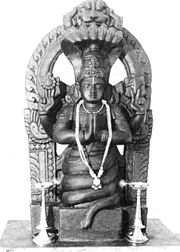
\includegraphics[width=0.5\linewidth,keepaspectratio]{images/yog15}
\end{center}

\begin{sanskrit}
योगेन चित्तस्य पदेन वाचां |
मलं शरीरस्य च वैद्यकेन |
योऽपाकरोक्तं प्रवरं मुनीनां |
पतञ्जलिं प्राञ्जलिरनतोस्मि ||
- राजा भर्तुहरि
\end{sanskrit}

    \end{column}
    \begin{column}[t]{0.6\linewidth}
		\begin{itemize}
	\item Patajali has been mentioned to have 3 contributions (two of them are lost in time)
	\item चित्तशुद्धि Purification of mind using Yog
	\item Purification of speech using Grammar
	\item Purification of body using medicine (Ayurveda)
	\item Better amongst sages, we salute Rishi Patanjali
	\end{itemize}

    \end{column}
  \end{columns}
\end{frame}


%%%%%%%%%%%%%%%%%%%%%%%%%%%%%%%%%%%%%%%%%%%%%%%%%%%%%%%%%%%
\begin{frame}[fragile]\frametitle{ योग सूत्र Yog Sutra}

	\begin{itemize}
	\item Sutra सूत्र Aphorisms, thread string धागा
	\item Minimum words, Unquestioned, Precise, essence, coherent eg. SthirSukhamAsan ( स्थिरसुखमासनम्| )
	\item Hard to understand by themselves so commentaries are needed.
	\item भाष्य commentaries starting with Vyas, are still going on (a living tradition)
	\item Vyasa's commentaries are highly regarded and have to be read along with Sutras.
	\end{itemize}

\tiny{(Ref: Patanjali Yoga Sutra Dr Mrudula Chaudhari)}

\end{frame}



%%%%%%%%%%%%%%%%%%%%%%%%%%%%%%%%%%%%%%%%%%%%%%%%%%%%%%%%%%%
\begin{frame}[fragile]\frametitle{Background}

	\begin{itemize}
	\item Patanjali Yog sutra emerged in the late Upanishad (उपनिषद) period
	\item Upanishads are earlier spiritual texts, but they are not systematic. They are mainly poetic expressions, metaphors some times confusing
	\item Examples: sometimes ब्रह्म साकार, sometimes ब्रह्म निराकार; जगन मिथ्या, जगन माया, जगन सत्य; आत्मन merges into ब्रह्मन्, etc). 
	\item Need to systematize.
	\end{itemize}

\tiny{(Ref: The Yoga Sutras of Patanjali | Prof. Edwin Bryant)}

\end{frame}

%%%%%%%%%%%%%%%%%%%%%%%%%%%%%%%%%%%%%%%%%%%%%%%%%%%%%%%%%%%
\begin{frame}[fragile]\frametitle{Systematization}

	\begin{itemize}
	\item Badarayana बादरायण codified unstructured Upanishad  उपनिषद texts.
	\item You get a few references to Yog in the Upanishads.
	\item Mentioned as techniques to attain ataman/brahman (आत्मन/ब्रह्मन्)
	\item Patanjali comes, systematizes and writes Yog Sutra (अथ अनुशाशन, continuing teachings of yog)
	\end{itemize}

\tiny{(Ref: The Yoga Sutras of Patanjali | Prof. Edwin Bryant)}

\end{frame}

%%%%%%%%%%%%%%%%%%%%%%%%%%%%%%%%%%%%%%%%%%%%%%%%%%%%%%%%%%%
\begin{frame}[fragile]\frametitle{Structure}

	\begin{itemize}
	\item Yogsutra has been divided into 4 chapters
	\item Total 195 verses/aphorisms
	\item Division:
		\begin{itemize}
		\item Samadhipad समाधिपाद 51
		\item Sadhanpad साधनपाद 55
		\item Vibhutipad विभूतिपाद 55
		\item Kaivalyapad कैवल्यपाद 34
		\end{itemize}	
	\end{itemize}

\tiny{(Ref: पातंजल योग सूत्र | Yog Darshan - Yoga And Ayurveda Science Youtube channel)}

\end{frame}

%%%%%%%%%%%%%%%%%%%%%%%%%%%%%%%%%%%%%%%%%%%%%%%%%%%%%%%%%%%
\begin{frame}[fragile]\frametitle{Contents}

Different Yogic methods for different types of people.

Types of people (prakruti प्रकृति ) in the world:

	\begin{itemize}
	\item High (uttam उत्तम ) : Already in almost pure mental state. Get success with very less efforts (sadhana !!!) 
	\item Medium (madhyam मध्यम )
	\item Low (adham अधम): Least pure mental state. Need vigorous discipline
	\end{itemize}
	
\tiny{(Ref: पातंजल योग सूत्र | Yog Darshan - Yoga And Ayurveda Science Youtube channel)}

\end{frame}

%%%%%%%%%%%%%%%%%%%%%%%%%%%%%%%%%%%%%%%%%%%%%%%%%%%%%%%%%%%
\begin{frame}[fragile]\frametitle{Contents}

Methods to attain yogic state based on type:


	\begin{itemize}
	\item Samadhipad समाधिपाद : , for uttam prakrti people, along with study (abhyas अभ्यास) and renunciation (vairagya वैराग्य)
	\item Sadhanpad साधनपाद : for adham prakriti people. Ashtang yog to get rid off miseries in life.
	\item Vibhutipad विभूतिपाद : After doing sadhana (dharana धारणा, dhyaan ध्यान, samadhi समाधि), one can get certain powers (siddhi सिद्धि, vibhuti विभूति). Recommends not get enamored by these powers.
	\item Kaivalyapad कैवल्यपाद : State of self detachment (moksh मोक्ष, mukti मुक्ति)
	\end{itemize}	

\tiny{(Ref: पातंजल योग सूत्र | Yog Darshan - Yoga And Ayurveda Science Youtube channel)}

\end{frame}


%%%%%%%%%%%%%%%%%%%%%%%%%%%%%%%%%%%%%%%%%%%%%%%%%%%%%%%%%%%
\begin{frame}[fragile]\frametitle{Calling the Call Center}
	\begin{itemize}
	\item Yog Sutra is a practice text, and not a knowledge text.
	\item The Knowledge part is covered in Sankhya darshan (साङ्ख्य दर्शन)
	\item It is assumed that you have gone through the knowledge texts before.
	\item Gita's yoga definition is ACTION oriented, whereas Patanjali definition is IN-ACTION oriented.
	\end{itemize}

\tiny{(Ref: The Yoga Sutras of Patanjali | Prof. Edwin Bryant)}

\end{frame}

% %%%%%%%%%%%%%%%%%%%%%%%%%%%%%%%%%%%%%%%%%%%%%%%%%%%%%%%%%%%
% \begin{frame}[fragile]\frametitle{Calling the Call Center}
	% \begin{itemize}
	% \item Calling to an IVR (Integrated Voice Response)
	% \item A pre-recorded menu selection.
	% \item ``Please press 1 for Account Details, Please press 2 for \ldots''
	% \item Till it comes to your option. 
	% \item Else, you are given access to a person to talk to.
	% \end{itemize}

% Boring? Annoying? But still heavily used \ldots, Why?

% \begin{center}
% \includegraphics[width=0.5\linewidth,keepaspectratio]{nlp10}

% \tiny{(Ref: Deep Learning and NLP A-Z - Kirill Eremenko)}
% \end{center}
% Instead, how about typing/saying your query directly and getting the answer right away?

% \end{frame}